\documentclass[border=0mm]{standalone}

\usepackage{import}
\subimport{../../../}{preamble.tex}

\usepackage{tikz}
\usetikzlibrary{calc}
\usepackage{pgfplots}
\usepgfplotslibrary{fillbetween}

\renewcommand{\t}{-5}

\begin{document}

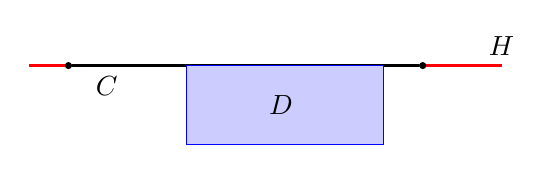
\begin{tikzpicture}
  
  \draw[line width=1pt, red] (-3, 0) -- (3, 0);
  \node[above] at (3, 0) {$\red{H}$};

  \node[circle, draw=black, fill=black, inner sep=0.75pt] (C_l) at (-2.5, 0) {};
  \node[circle, draw=black, fill=black, inner sep=0.75pt] (C_u) at (+2, 0) {};
  \draw[line width=1pt] (C_l) -- (C_u) node[pos=0.1, below] {$C$};

  \draw[draw=blue, fill=blue!20] (-1, 0) -- (1.5, 0) -- (1.5, -1) -- (-1, -1) -- cycle;
  \node[] at (0.2, -0.5) {$D$};

  
\end{tikzpicture}

\end{document}

%%% Local Variables:
%%% mode: latex
%%% TeX-master: t
%%% End:
